\documentclass[aspectratio=169]{beamer}
\usepackage{graphicx}
\usepackage[english]{babel}
\usepackage{tikz}
\usepackage{pgfplots}
\pgfplotsset{compat=1.18}
\usepackage{booktabs}
\usetikzlibrary{shapes.geometric, arrows}
\tikzstyle{block} = [rectangle, rounded corners, minimum width=3cm, minimum height=1cm,text centered, draw=black, fill=blue!20]
\tikzstyle{arrow} = [thick,->,>=stealth]
\usepackage{pgf-pie}

\usetheme[sectionpage=progressbar, progressbar=frametitle]{metropolis}
\title{Quantum Enhanced Machine Learning}
\subtitle{Sentiment Analysis Approach}
\author{Mario Bifulco, Luca Roversi}
\date{University of Turin}
\institute{mario.bifulco@edu.unito.it, luca.roversi@unito.it}

\begin{document}
\setbeamertemplate{section in toc}[sections numbered]

\begin{frame}
    \titlepage
\end{frame}

\begin{frame}
    \frametitle{Goal}

    Testing the effectiveness of quantum computation on machine learning tasks

    \vspace{1cm}

    Using the QPU extensively while avoiding the closed source alternatives of D-Wave

\end{frame}

\begin{frame}
    \frametitle{Applying Quantum Annealing to Sentiment Analysis}

    \only<1>{
        \begin{exampleblock}{Quantum Annealing}
            QA is an optimization process for finding the global minimum of a given objective function over a given set of candidate solutions.
        \end{exampleblock}
    }

    \only<2>{
        \begin{exampleblock}{Quantum Annealing}
            QA is an optimization process for finding the global minimum of a given objective function over a given set of candidate solutions.
        \end{exampleblock}

        \begin{exampleblock}{Sentiment Analysis}
            SA is the use of natural language processing to systematically identify, extract, quantify, and study affective states and subjective information.      
        \end{exampleblock}
    }

    \only<3>{
        \begin{exampleblock}{Quantum Annealing}
            QA is an optimization process for finding the global minimum of a given objective function over a given set of candidate solutions.
        \end{exampleblock}

        \begin{exampleblock}{Sentiment Analysis}
            SA is the use of natural language processing to systematically identify, extract, quantify, and study affective states and subjective information.      
        \end{exampleblock}

        \begin{exampleblock}{Goal of Machine Learning}
            Minimizing a loss function.
        \end{exampleblock}
    }

\end{frame}

\begin{frame}
    \frametitle{From Machine Learning to Quantum Annealing}
    
    \centering
    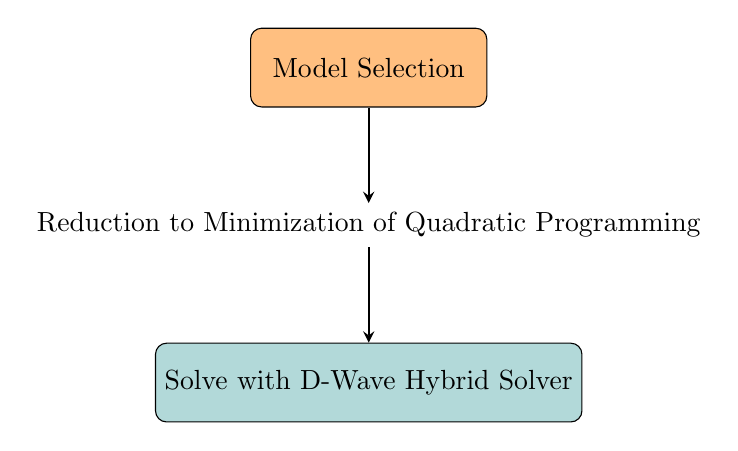
\begin{tikzpicture}[node distance=2cm]
        \node (step1) [block, fill=orange!50] {Model Selection};
        \node (step2) [below of=step1] {Reduction to Minimization of Quadratic Programming};
        \node (step3) [block, below of=step2, fill=teal!30] {Solve with D-Wave Hybrid Solver};
    
        \draw [arrow] (step1) -- (step2);
        \draw [arrow] (step2) -- (step3);
    \end{tikzpicture}

\end{frame}

\begin{frame}
    \frametitle{Binary Sentiment Analysis Results}

    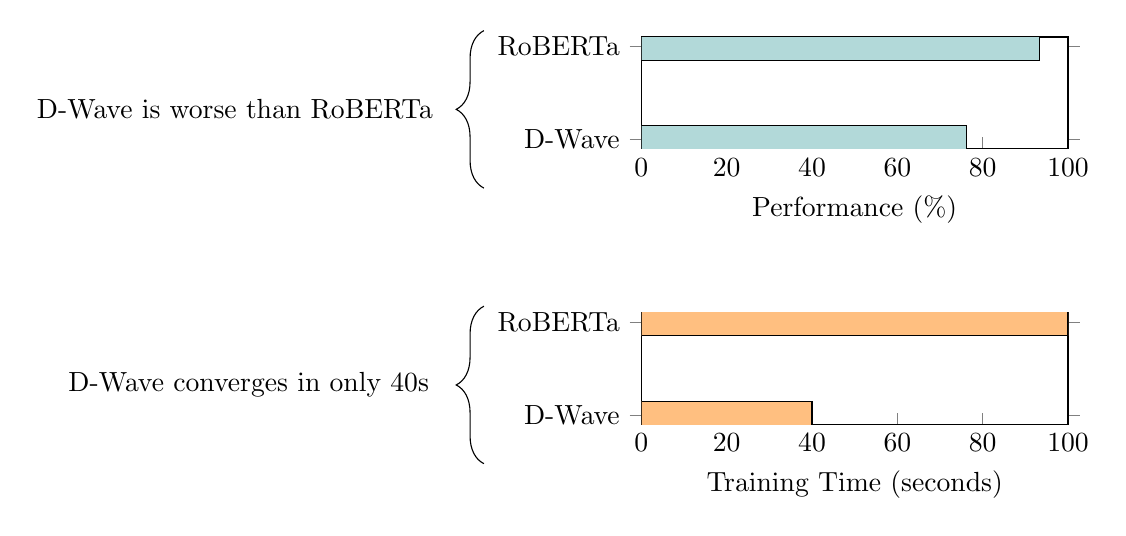
\begin{tikzpicture}
        \draw[decorate,decoration={brace,amplitude=10pt}] (-2,-0.5) -- (-2,1.5) node [black,midway,xshift=-90pt] {D-Wave is worse than RoBERTa};
        \begin{axis}[
            width=7cm, height=3cm,
            xbar, bar width=10pt,
            symbolic y coords={D-Wave,RoBERTa},
            ytick=data,
            xlabel={Performance (\%)},
            xmin=0, xmax=100,
            ]
            \addplot[fill=teal!30] coordinates {(93.4,RoBERTa) (76.1,D-Wave)};
        \end{axis}
        
        \draw[decorate,decoration={brace,amplitude=10pt}] (-2,-4) -- (-2,-2) node [black,midway,xshift=-85pt] {D-Wave converges in only 40s};
        \begin{axis}[
            yshift=-3.5cm,
            width=7cm, height=3cm,
            xbar, bar width=10pt,
            symbolic y coords={D-Wave,RoBERTa},
            ytick=data,
            xlabel={Training Time (seconds)},
            xmin=0, xmax=100,
            ]
            \addplot[fill=orange!50] coordinates {(100,RoBERTa) (40,D-Wave)};
        \end{axis}
    \end{tikzpicture}

\end{frame}

\begin{frame}
    \frametitle{Usage of QPU to Obtain the Above BSA}

    \begin{columns}
        \begin{column}{0.5\textwidth}
            \centering
            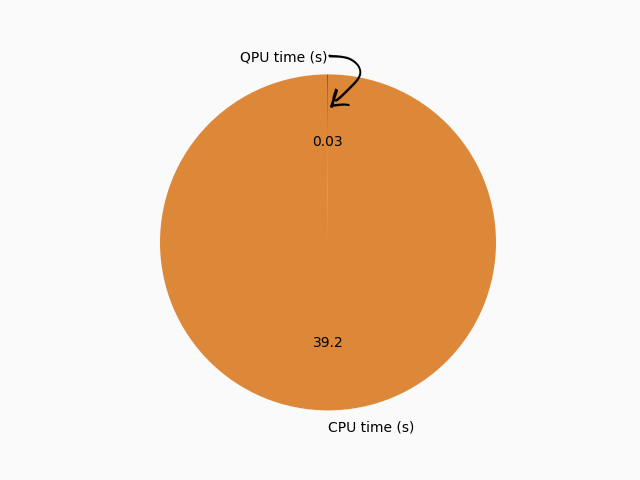
\includegraphics[height=0.65\textheight]{img/piechart2.png}
        \end{column}
        \begin{column}{0.5\textwidth}
            \begin{itemize}
                \item Only 0.08\% of the time is spent on the QPU
                \item The performance boost should comes from quantum annealing
                \item Is it possible to increase the QPU usage?
                \item Is it possible to avoid the closed-source procedures of D-Wave?
            \end{itemize}
        \end{column}
        
    \end{columns}

\end{frame}

\begin{frame}
    \frametitle{From Quadratic Problem to QPU}

    \only<1>{
        \centering
        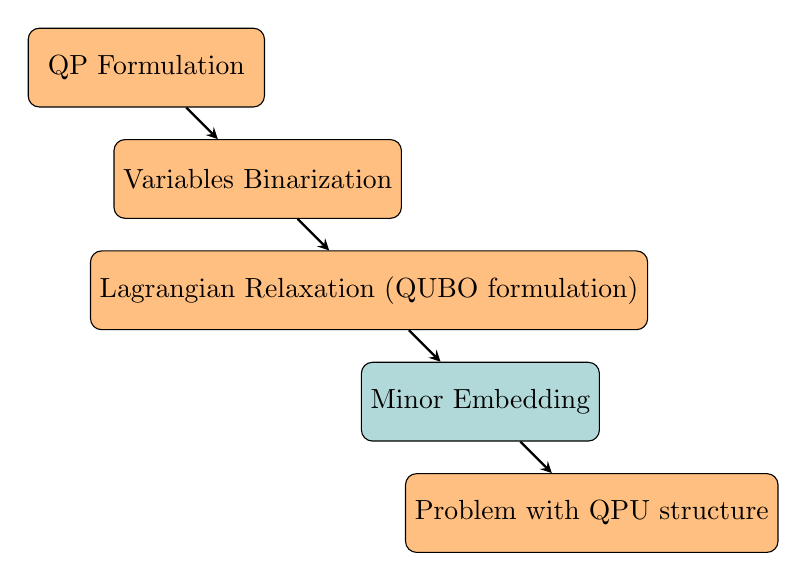
\begin{tikzpicture}[node distance=2cm]
            \node (step1) [block, fill=orange!50] {QP Formulation};
            \node (step2) [block, below right of=step1, fill=orange!50] {Variables Binarization};
            \node (step3) [block, below right of=step2, fill=orange!50] {Lagrangian Relaxation (QUBO formulation)};
            \node (step4) [block, below right of=step3, fill=teal!30] {Minor Embedding};
            \node (step5) [block, below right of=step4, fill=orange!50] {Problem with QPU structure};
        
            \draw [arrow] (step1) -- (step2);
            \draw [arrow] (step2) -- (step3);
            \draw [arrow] (step3) -- (step4);
            \draw [arrow] (step4) -- (step5);
        \end{tikzpicture}
    }

    \only<2>{
        \begin{columns}
            \begin{column}{0.4\textwidth}
                SVM graph for 8 variables
            \end{column}
            \begin{column}{0.1\textwidth}
                \LARGE
                $\Longrightarrow$
            \end{column}
            \begin{column}{0.4\textwidth}
                Mapped problem on Pegasus QPU
            \end{column}
        \end{columns}
        \vspace{0.5cm}
        \begin{columns}
            \begin{column}{0.4\textwidth}
                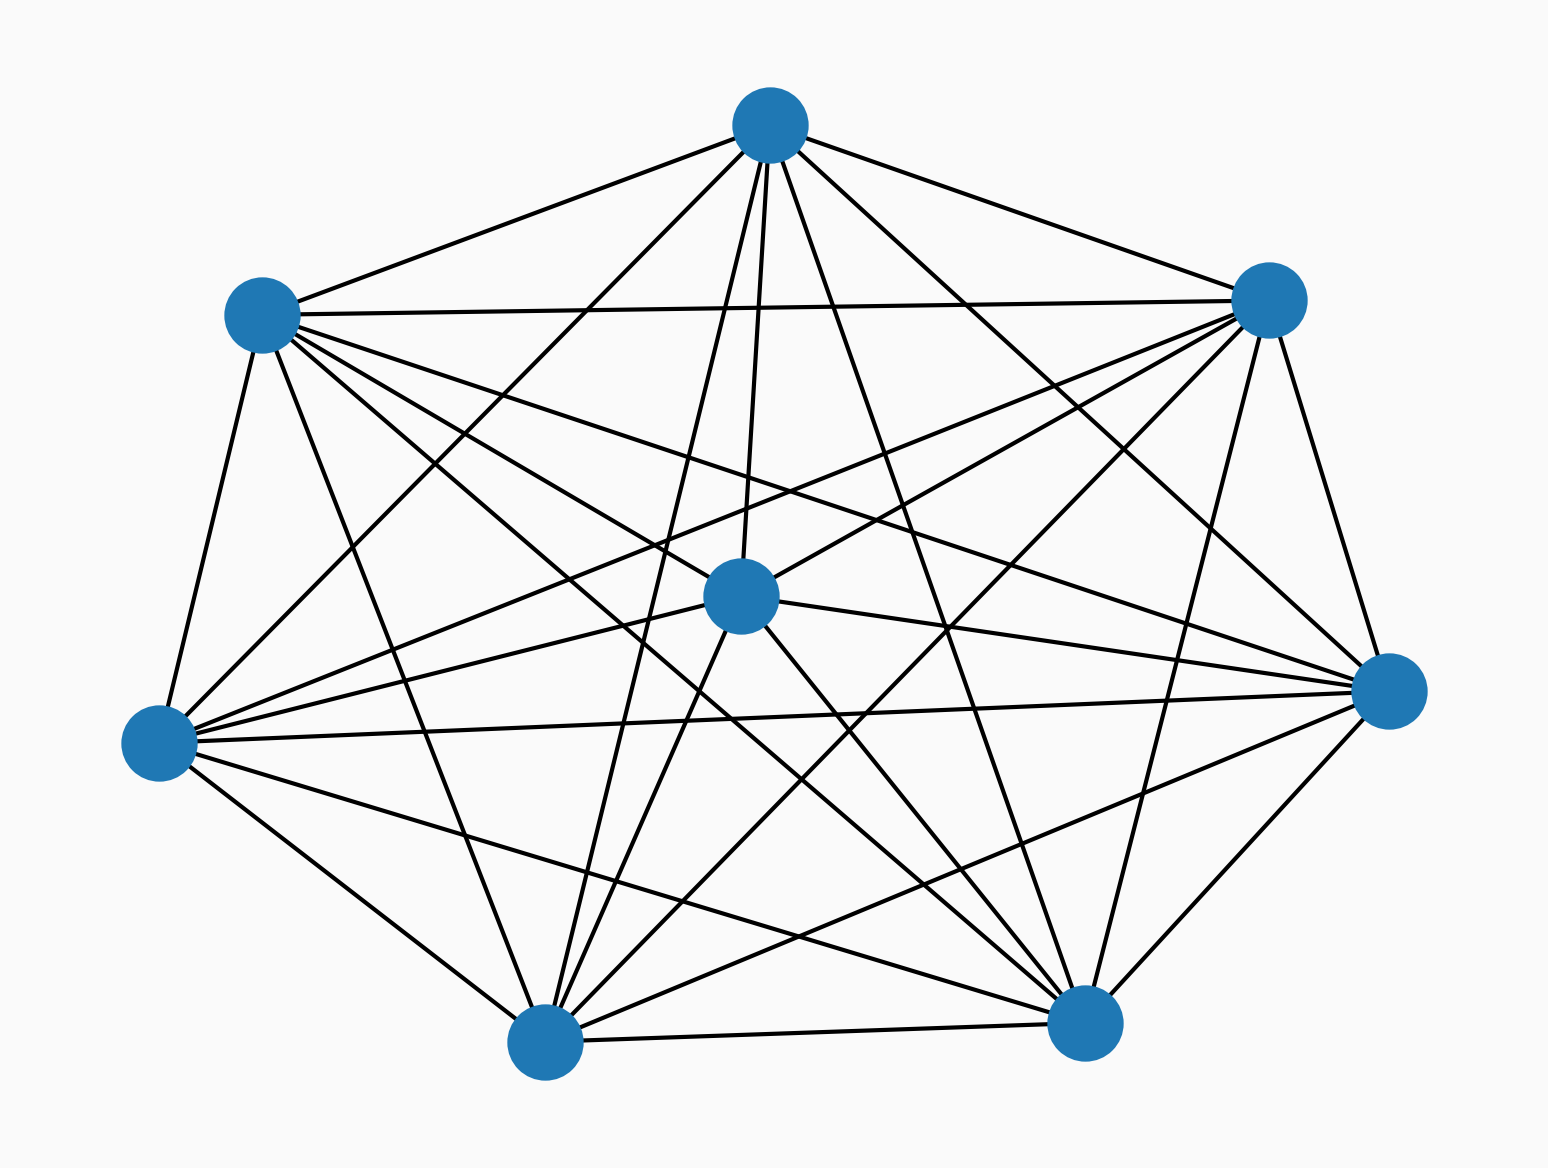
\includegraphics[width=\textwidth]{img/source.png}
            \end{column}
            \begin{column}{0.1\textwidth}
                \LARGE
                $\Longrightarrow$
            \end{column}
            \begin{column}{0.4\textwidth}
                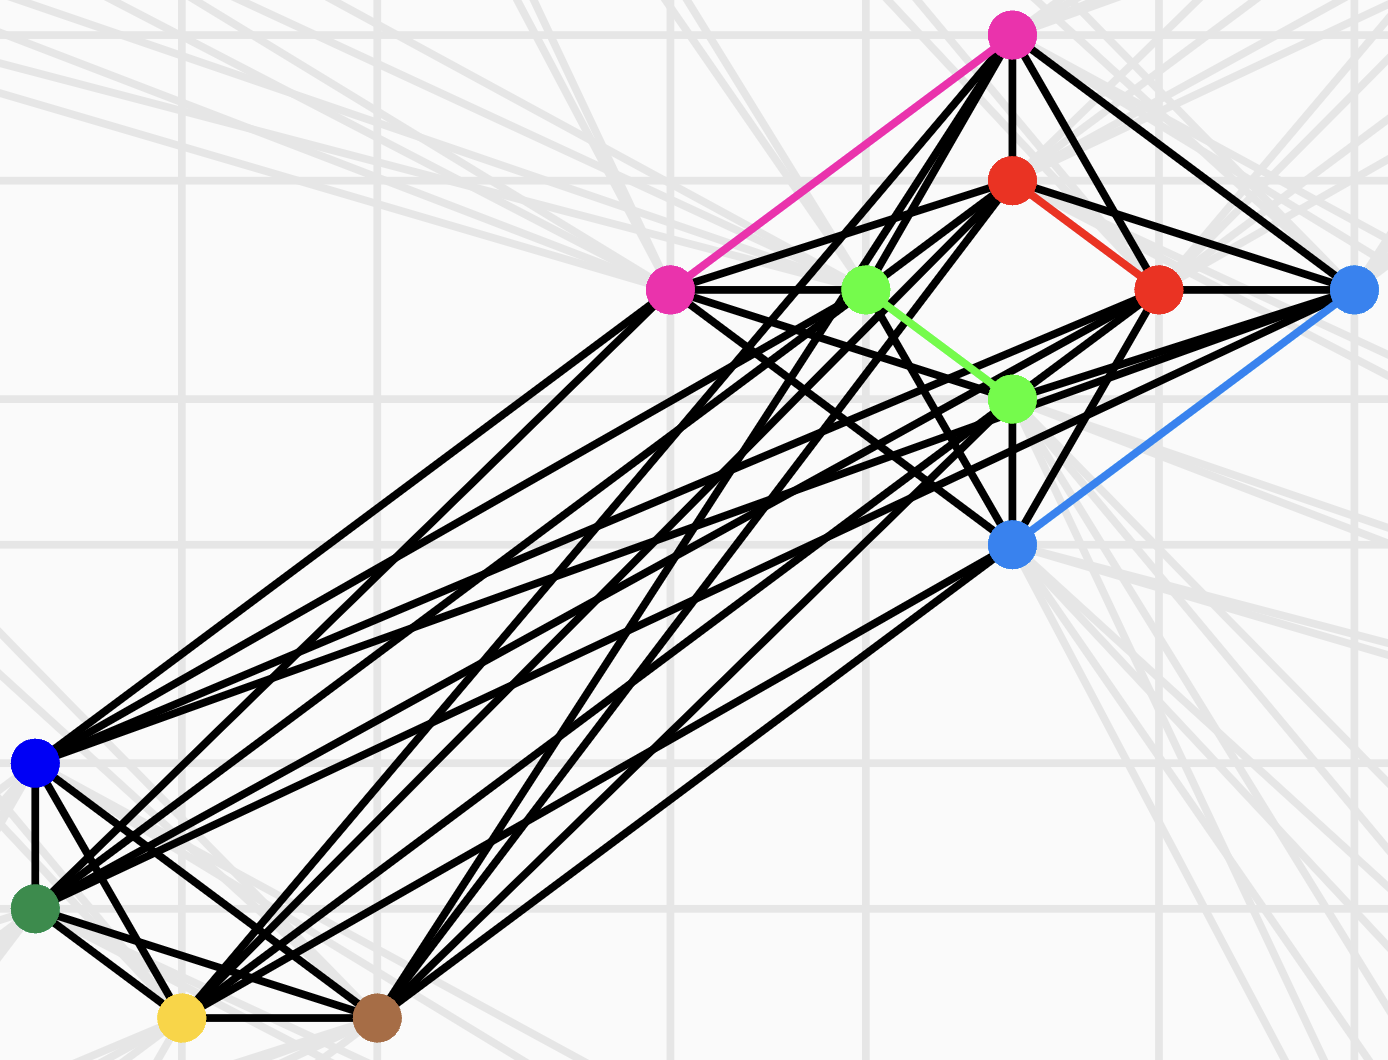
\includegraphics[width=\textwidth]{img/target.png}
            \end{column}
        \end{columns}
    }

\end{frame}

\begin{frame}
    \frametitle{Pegasus QPU is not enough}

    \begin{columns}
        \begin{column}{0.5\textwidth}
            For SVMs with 128 binary variables, the QPU is almost completely used
        \end{column}
        \begin{column}{0.5\textwidth}
            \centering
            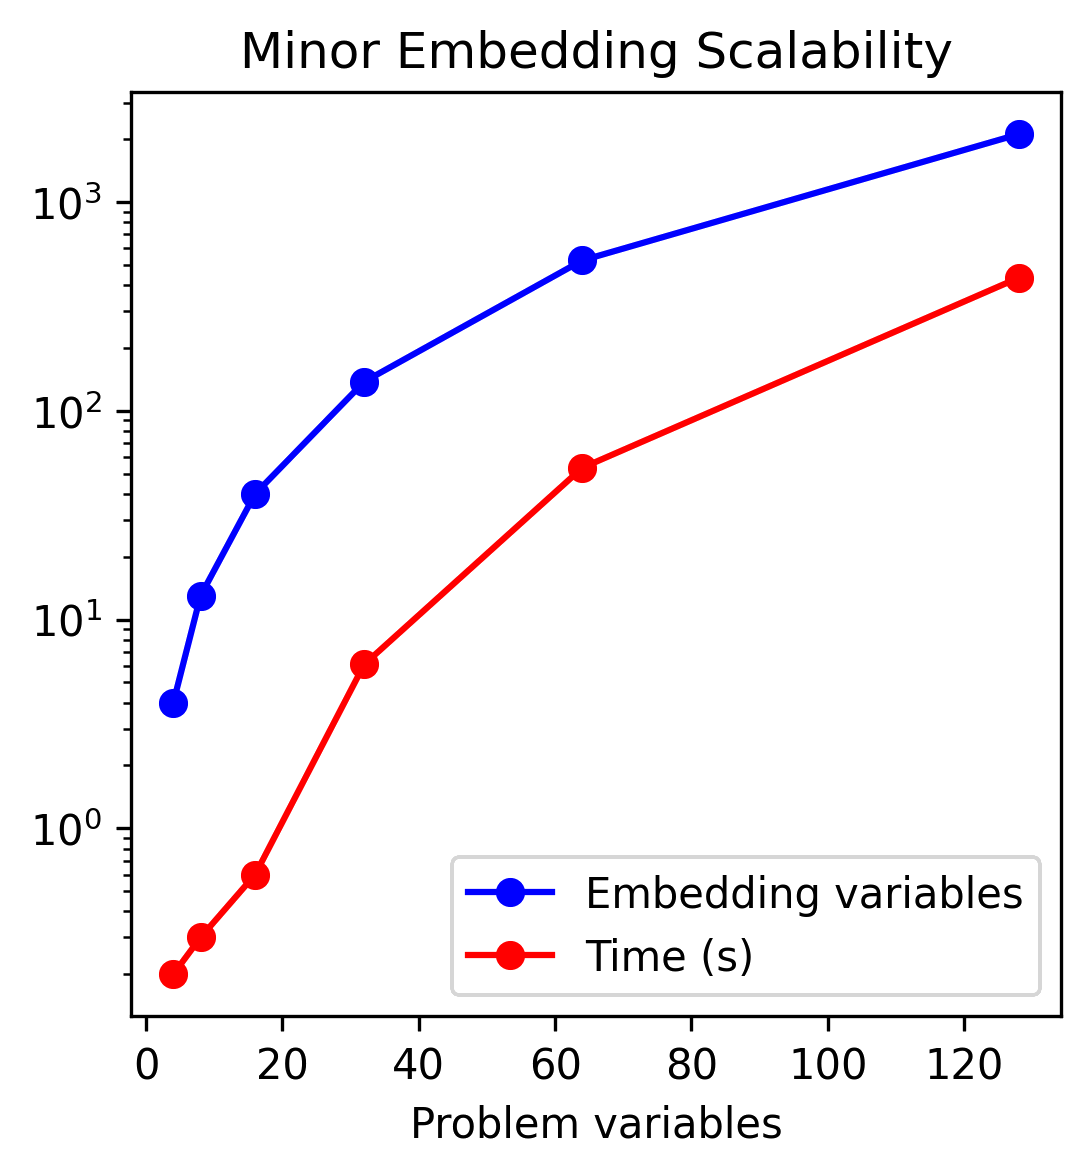
\includegraphics[height=0.8\textheight]{img/embedding_search_time.png}
        \end{column}
    \end{columns}

\end{frame}

\begin{frame}
    \frametitle{QUBO Formulation}

    The QPU process directly problems in QUBO form:

    $$\arg\min_x x^TQx$$
    $$x_i \in \{0, 1\} \forall i$$

    Example with 4 binary variables:

    \begin{center}         
        $\begin{bmatrix}
          x_1 & x_2 & x_3 & x_4
        \end{bmatrix}$
        $\begin{bmatrix}
          -3 & 5 & 1 & -7 \\
          0 & 1 & 0 & 8 \\
          0 & 0 & 9 & -4 \\
          0 & 0 & 0 & -2 
        \end{bmatrix}$
        $\begin{bmatrix}
          x_1 \\ x_2 \\ x_3 \\ x_4
        \end{bmatrix}$      
    \end{center}

\end{frame}

\begin{frame}
    \frametitle{\texttt{QSplitSampler} - Problem Splitting}

    \centering
    \begin{tikzpicture}[node distance=6cm]        
        \node (step1) {            
            \begin{tikzpicture}
                \draw (1.5,3.3) node {Initial problem};
                \draw (0,0) rectangle (3,3);
                \fill[gray!90, opacity=0.75] (3, 0) -- (0, 0) -- (0, 3) -- cycle;
            \end{tikzpicture}
        };

        \node (step2) [right of=step1] {            
            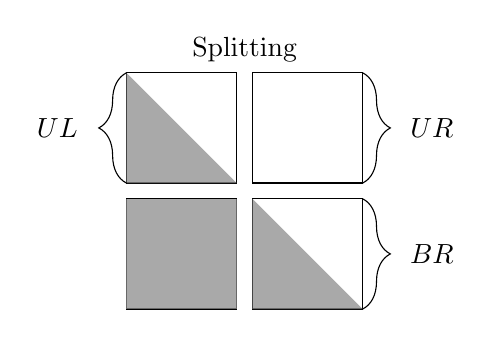
\begin{tikzpicture}
                \draw (1.5,3.3) node {Splitting};
                \draw (0,0) rectangle (1.4,1.4);
                \draw (1.6,1.6) rectangle (3,3);
                \draw (0,1.6) rectangle (1.4,3);
                \draw (1.6,0) rectangle (3,1.4);
                \fill[gray!90, opacity=0.75] (0,0) -- (0,1.4) -- (1.4,1.4) -- (1.4,0);
                \fill[gray!90, opacity=0.75] (0,1.6) -- (0,3) -- (1.4,1.6) -- cycle;
                \fill[gray!90, opacity=0.75] (1.6,0) -- (3,0) -- (1.6,1.4) -- cycle;
    
                \draw[decorate,decoration={brace,amplitude=10pt}] (0,1.6) -- (0,3) node [black,midway,xshift=-25pt] {$\operatorname{UL}$};
                \draw[decorate,decoration={brace,amplitude=10pt,mirror}] (3,1.6) -- (3,3) node [black,midway,xshift=25pt] {$\operatorname{UR}$};
                \draw[decorate,decoration={brace,amplitude=10pt,mirror}] (3,0) -- (3,1.4) node [black,midway,xshift=25pt] {$\operatorname{BR}$};
            \end{tikzpicture}
        };

        \draw [arrow] (step1) -- (step2);
    \end{tikzpicture}

\end{frame}

\begin{frame}
    \frametitle{\texttt{QSplitSampler} - Solving Subproblems}

    \centering
    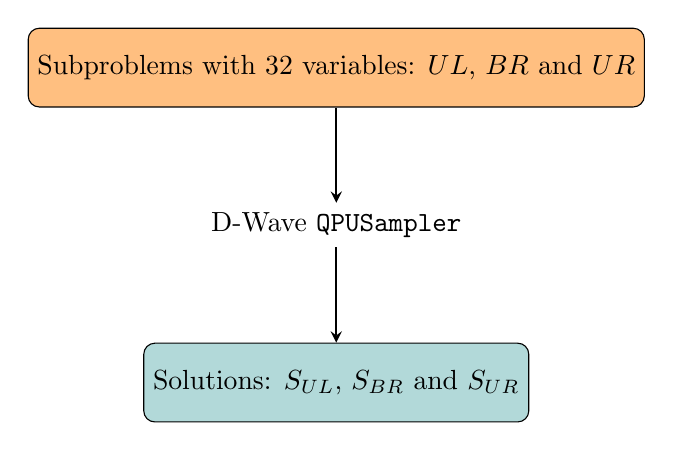
\begin{tikzpicture}[node distance=2cm] 
        \node (step1) [block, fill=orange!50] {
            Subproblems with 32 variables: $\operatorname{UL}$, $\operatorname{BR}$ and $\operatorname{UR}$
        };

        \node (step2) [below of=step1] {
            D-Wave \texttt{QPUSampler}
        };

        \node (step3) [block, below of=step2, fill=teal!30] {
            Solutions:

            $\operatorname{S_{UL}}$, $\operatorname{S_{BR}}$ and $\operatorname{S_{UR}}$
        };

        \draw [arrow] (step1) -- (step2);
        \draw [arrow] (step2) -- (step3);
    \end{tikzpicture}
    
\end{frame}

\begin{frame}
    \frametitle{\texttt{QSplitSampler} - Aggregate Solutions}

    \centering
    Aggregating $\operatorname{S_{UL}}$, $\operatorname{S_{BR}}$ and $\operatorname{S_{UR}}$ gives two sets of variables

    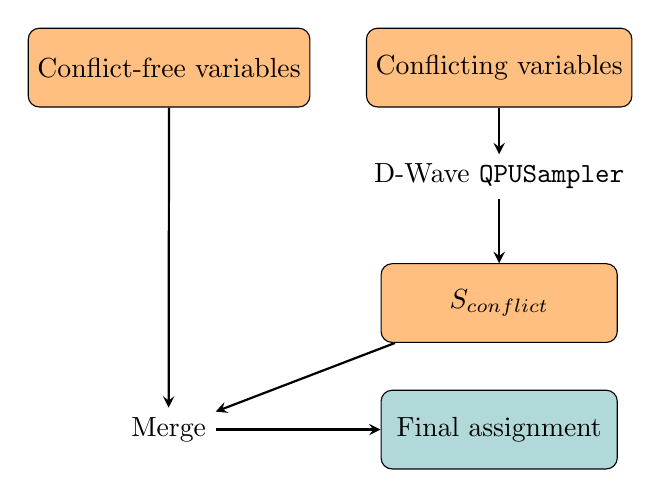
\begin{tikzpicture}[node distance=1cm] 
        \node (step1) [block, fill=orange!50] {
            Conflict-free variables
        };

        \node (step2) [block, right of=step1, right=1.5cm, fill=orange!50] {
            Conflicting variables
        };

        \node (step3) [below of=step2, below=0.1cm] {
            D-Wave \texttt{QPUSampler}
        };

        \node (step4) [block, below of=step3, below=0.1cm, fill=orange!50] {
            $S_{conflict}$
        };

        \node (step5) [block, below of=step4, below=0.1cm, fill=teal!30] {
            Final assignment
        };

        \node (step6) [left of=step5, left=2.6cm] {
            Merge
        };

        \draw [arrow] (step1) -- (step6);
        \draw [arrow] (step6) -- (step5);
        \draw [arrow] (step2) -- (step3);
        \draw [arrow] (step3) -- (step4);
        \draw [arrow] (step4) -- (step6);
    \end{tikzpicture}

\end{frame}

\begin{frame}
    \frametitle{\texttt{QSplitSampler} Results}

    \begin{table}
        \centering
        \begin{tabular}{ccc|cc}
            \toprule
            \multicolumn{3}{c}{\texttt{QSplitSampler}} & \multicolumn{2}{c}{\texttt{QPUSampler}} \\
            Cut Dim         & Classical time & QPU time & Classical time & QPU time \\
            \midrule
            2               & 470.71 & 0.45     & 142.54 & 0.02 \\
            4               & 223    & 0.35     & 116.02 & 0.02 \\
            8               & 94.97  & 0.25     & 271.36 & 0.02 \\
            16              & 68.33  & 0.17     & 190.29 & 0.02 \\
            32              & 48.46  & 0.1      & 207.86 & 0.02 \\
            \bottomrule
        \end{tabular}
        \caption{Results for randomly generated QUBO problems with 128 variables}
    \end{table}

\end{frame}

\begin{frame}
    \frametitle{Conclusion}

    Using only the \textbf{free version} of the D-Wave solvers, we showed:

    \begin{itemize}
        \item How hybrid solvers can be used for real problems
        \item How closed source infrastructure can be avoided
        \item How the use of QPU can be increased
    \end{itemize}

    \vspace{1cm}

    Does this bring benefits when solving machine learning problems?

\end{frame}

\section{Thanks for your attention}

\end{document}